\documentclass{beamer}
\usepackage{ctex} %注意这个宏包
\usepackage{multicol}
\usepackage{color}
\usepackage{graphics,graphicx}
\usepackage{listings}
\usepackage{amsmath}
%\usetheme{umbc4}
%\usetheme[height=12mm]{Rochester}
%\usetheme{Marburg}
\usetheme{Berkeley}
\useinnertheme{umbcboxes}
\definecolor{almond}{rgb}{0.94, 0.87, 0.8}
%\useinnertheme{rounded}
\CTEXoptions[today=old]
%\setbeamercolor{beaver}{bg=violet!15,fg=black}  % redefine box color!

\title{wbia 实验报告}
\author{Chunwei Yan}
\institute[PKUSZ]{
\texttt{YanChunwei@outlook.com}
}
\date{\today}

\begin{document}
% ------------- title page ----------------------------
%--- the titlepage frame -------------------------%
\begin{frame}
  \titlepage
\end{frame}

% -------------- outline ------------------------------
\section{Begin}
\begin{frame}
\frametitle{Outline}
\tableofcontents
\end{frame}
\subsection{实验内容}
\begin{frame}
\frametitle{实验内容}
    \begin {itemize} 
    \item 网页模板检测
    \pause
    \item SST (Site Style Tree) 算法
    \pause
    \item 爬取网页测试
    \pause
    \item 可视化的测试结果
    \pause
    \end{itemize}
\end{frame}

\subsection{实验环境}
\begin{frame}{实验环境}
    \begin{itemize}
    \item Python2.7
        \begin{description}[Second Item]
        \pause
        \item [PyQuery] 网页解析
    \pause
        \item [Numpy] 数值计算
        \end{description}
    \pause
    \item Linux Mint
    \pause
    \item 数据来源: news.MSN.com, news.yahoo.com
    \end{itemize}
\end{frame}

\section{SST 算法}
\begin{frame}{SST 算法}
    \begin{center}
    \includegraphics[height=5cm]{sst_structure.png}
    \end{center}
    \pause
    \begin{itemize}
        \item element node , style node
    \pause
        \item {\color{blue} leaf node}
    \end{itemize}
\end{frame}

\subsection{具体实现}
\begin{frame}{一些设定}
    \begin{center}
    \begin{overprint}
        \onslide<1>
        \begin{block}{数据结构}
            \begin{description}[Second Item]
                \item [ElementNode] 普通节点
                \item [StyleNode] 父节点的直系子节点的起始标签
                \item [DataNode] ElementNode的feature内容
                \item [StyleTree] 包含一个Body-ElementNode
            \end{description}
        \end{block}

        \onslide<2>
        \begin{block}{Demo}
            \begin{center}
            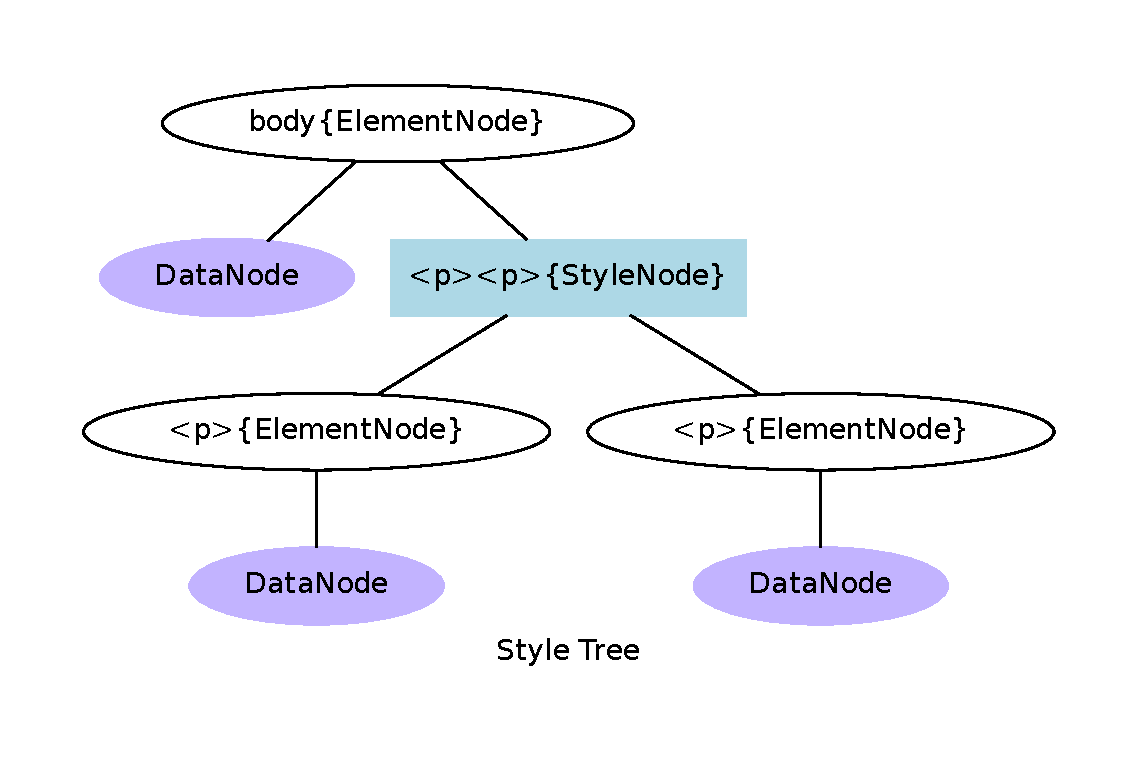
\includegraphics[height=5cm]{../dot/data_structure_demo.pdf}
            \end{center}
        \end{block}
    \end{overprint}
    \end{center}
\end{frame}

\begin{frame}{一些设定}
    \begin{center}
    \begin{overprint}
        \onslide<1>
        \begin{block}{细节定义}
            \begin{description}[Second Item]
            \item [features] words and special tags
                \begin{itemize}
                \item word
                \item tags: A IMG 
                \end{itemize}
            \item [leaf node] 仅包含DataNode的节点
            \end{description}
        \end{block}

        \onslide<2>
        \begin{block}{Demo}
            \begin{center}
            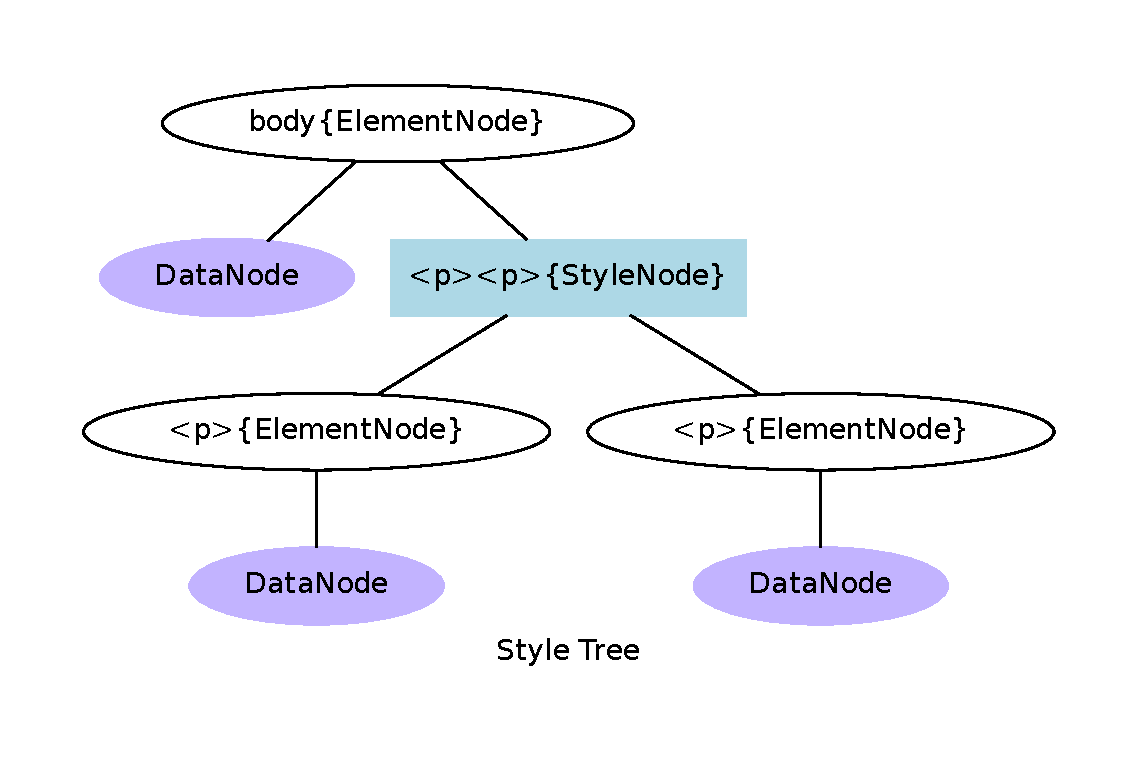
\includegraphics[height=5cm]{../dot/data_structure_demo.pdf}
            \end{center}
        \end{block}
    \end{overprint}
    \end{center}
\end{frame}
\subsection{算法思考}
\begin{frame}{存在问题?}
    %介绍计算方法
    %存在问题
    \begin{block}{Element(非leaf node)权重计算}
        {\zihao{6}{
        $$
        CompImp_{former}(E) = (1-r')NodeImp(E) + r' \sum_{i=1}^{l}{p_iCompImp(s_i)}
        $$}
        $$
        CompImp(S_i) = \frac{
                \sum_{j=1}^{k}{CompImp(E_j)}
            } {k}
        $$
        \pause
        $$
        NodeImp(E) = 
        \begin{cases}
            \begin{array}{ll}
                -\sum_{i=1}^{l}{p_i\log_{m}{p_i}} & if \quad m>1\\
                1                                   & if \quad m=1\\
            \end{array}    
        \end{cases}
        $$}
        \pause
        \begin{description}
        \item [$NodeImp(E)$] 拥有的风格样式(StyleNode)的熵
        \item [$CompImp(S_i)$] 子孙节点权重的传递
        \end{description}
    \end{block}
\end{frame}

\begin{frame}{存在问题?}
    %介绍计算方法
    %存在问题
    \begin{block}{Element(非leaf node)权重计算}
        {\zihao{6}{
        $$
        CompImp_{former}(E) = (1-r')NodeImp(E) + r' \sum_{i=1}^{l}{p_iCompImp(s_i)}
        $$}
        $$
        CompImp(S_i) = \frac{
                \sum_{j=1}^{k}{CompImp(E_j)}
            } {k}
        $$
        $$
        NodeImp(E) = 
        \begin{cases}
            \begin{array}{ll}
                -\sum_{i=1}^{l}{p_i\log_{m}{p_i}} & if \quad m>1\\
                1                                   & if \quad m=1\\
            \end{array}    
        \end{cases}
        $$}
        \begin{center}
        \begin{overprint}
        \onslide<1>
        \begin{description}
        \item [$NodeImp(E)$] 拥有的风格样式(StyleNode)的熵
        \item [$CompImp(S_i)$] 子孙节点权重的传递
        \end{description}
        \onslide<2>
        \begin{alertblock}{忽略非叶子节点的feature}
        \end{alertblock}
        \end{overprint}
        \end{center}
    \end{block}
\end{frame}


\begin{frame}{问题演示}
    \begin{center}
    \begin{overprint}
    \onslide<1>
    \begin{block}{Source Code Demo}
        \begin{center}
        \includegraphics[height=2cm]{ignore_data_of_node.png}
        \end{center}
    \end{block}
    \onslide<2>
    \begin{block}{Html Node Tree Demo}
        \begin{center}
        \includegraphics[height=5.5cm]{../dot/ignore_data_of_node.pdf}
        \end{center}
    \end{block}
    \onslide<3>
    \begin{block}{Our Practice}
        \begin{center}
        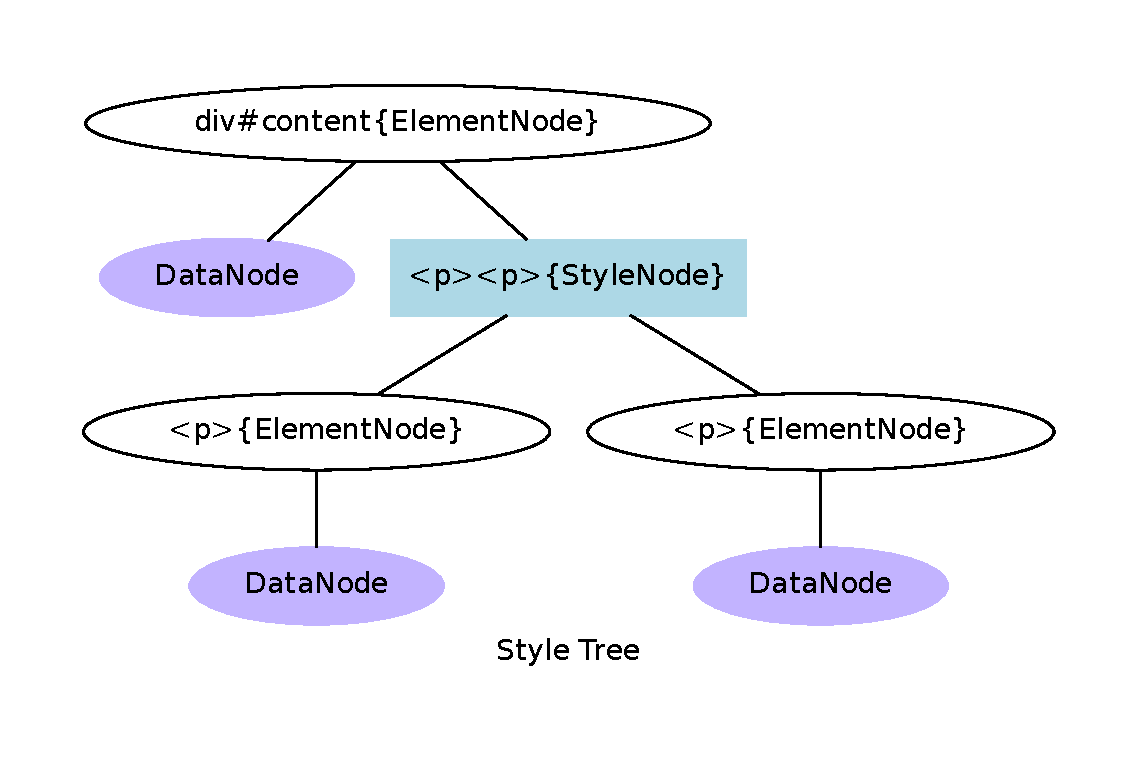
\includegraphics[height=5.5cm]{../dot/ignore_data_of_node_solution.pdf}
        \end{center}
    \end{block}
    \end{overprint}
    \end{center}
\end{frame}

\begin{frame}{算法思考}
    \begin{block}{重要性分配}
    \begin{center}
    \begin{overprint}
        \onslide<1>
        看作为叶子节点计算其内容feature的重要性
        {\zihao{6}{
        $$
        DataImp(E) = CompImp_{leaf}(E) = 
        \begin{cases}
            \begin{array}{ll}
            1 & if\quad m=1\\
            1 - \frac{ \sum_{i=1}^{l}{H(a_i)} }{l} & if \quad m>1\\
            \end{array}
        \end{cases}
        $$
        $$
        H(a_i) = - \sum_{j=1}^{m}{p_{ij}\log_{m}{p_{ij}}}
        $$
        }}
        \onslide<2>
        将内容feature的重要性与其原来的重要性以一定比例中和
        {\zihao{6}{
        $$
        CompImp_{former}(E) = (1-r')NodeImp(E) + r' \sum_{i=1}^{l}{p_iCompImp(s_i)}
        $$
        $$
        CompImp_{final}(E) = (1 - k)CompImp_{former}(E) + k*DataNode(E) 
        $$
        $$
        k = \frac{DataNode(E)}{
                CompImp_{former}(E) + DataNode(E)
            }
        $$
        }}
    \end{overprint}
    \end{center}
    \end{block}
\end{frame}

\section{测试及结果}

\subsection{SST结构实现演示}
\begin{frame}{SST结构测试}
    %一个简单的树形图
    \includegraphics[height=2cm]{sst_self_2.png}
\end{frame}

\begin{frame}{测试环境}
    %一个简单的树形图
    \begin{enumerate}
        \item news.MSN.com 650页 4轮
        \begin{itemize}
            \item 0.33
            \item 0.2
            \item 0.4
            \item 0.5
        \end{itemize}
                \pause
        \item news.yahoo.com 667页 2轮 对比
        \begin{itemize}
            \item 原始算法
            \item 为普通element node加入features权重
        \end{itemize}
    \end{enumerate}
\end{frame}

\subsection{实例演示}
\begin{frame}{实验数据}
    %实验数据 图片展示
    \fbox{from}
    \begin{center}
    \includegraphics[height=6cm]{old_page.png}
    \end{center}
\end{frame}
\begin{frame}{实验数据1}
    %实验数据 图片展示
    \fbox{to} $t= 0.33$
    \begin{center}
    \includegraphics[height=6cm]{0.33_image}
    \end{center}
\end{frame}
\begin{frame}{实验数据1}
    %实验数据 图片展示
    \fbox{to} $t= 0.2$
    \begin{center}
    \includegraphics[height=6cm]{0.2_image}
    \end{center}
\end{frame}
\begin{frame}{实验数据1}
    %实验数据 图片展示
    \fbox{to} $t= 0.4 or 0.5$
    \begin{center}
    \includegraphics[height=6cm]{0.4_0.5_image}
    \end{center}
\end{frame}
\begin{frame}{实验数据2}
    %实验数据 图片展示
    \fbox{from} news.yahoo, 原始算法 $t=0.33$
    \begin{center}
    \includegraphics[height=6cm]{yahoo_news1.5_image}
    \end{center}
\end{frame}
\begin{frame}{实验数据2}
    %实验数据 图片展示
    \fbox{from} news.yahoo, 加入feature
    \begin{center}
    \includegraphics[height=6cm]{yahoo_news_adddata.5_image}
    \end{center}
\end{frame}

\section{End}
\begin{frame}{不足及后续}
    \begin{enumerate}
    \item html解析 (PyQuery or Webkit ...?)
    \item 评测的严谨性
    \item 算法思考
    \end{enumerate}
\end{frame}
\begin{frame}{Goodbye}
    \begin{center}
    \fbox{\zihao{1} Tankyou }
    \end{center}
\end{frame}

\end{document}


